%!TEX root=../document.tex

\section{Ergebnisse}
\label{sec:Ergebnisse}

\subsection{CORBA Grundlagen}
CORBA steht f\"ur Common Object Request Broker Architecture und ist eine standardisierte Spezifikation einer Middleware f\"ur verteilte Objektaufrufe.
Im Gegensatz zu RMI ist CORBA Programmiersprachenunabh\"angig, so kann beispielsweise der Client in C++ und der Server in Java programmiert werden.
In folgender Graphik bietet einen \"Uberblick \"uber die Komponenten einer Client-Server Andwendung in CORBA.

\begin{figure}[H]
	\begin{center}
		\includegraphics[width=0.6\linewidth]{images/corba.pdf}
		\caption{Corba Client-Server Beispiel\cite{corba-client-server}}
		\label{broker}
	\end{center}
\end{figure}

Ein wichtiges Element ist das IDL (Interface Definition Language).
Hierbei handelt es sich um eine Interfacedefinition, die sowohl der (also der Benutzer) also auch der Server (der Anbieter eines Remote Objekts) verwenden.

In der folgenden Graphik sind die verschienden Komponenten von CORBA dargestellt.
\begin{figure}[H]
	\begin{center}
		\includegraphics[width=0.5\linewidth]{images/corba.jpg}
		\caption{\"Ubersicht der Komponenten von CORBA \cite{corba-components}}
		\label{broker}
	\end{center}
\end{figure}

Wichtig hierbei sind die Stubs und Skeletons, sowie das ORB-Interface (Object Request Broker) und der Portable Object Adapter (POA).
Letzterer dient zum Export von Remote Objekten und zum Binden an den Namensdienst.

\subsection{Installation von JacOrb\cite{jacorb} und OmniORB\cite{omniorb}}
Die Durchf\"uhrung der Aufgabe erfolgte in einer virtuellen Maschiene auf Basis von Debian 8.3 Jessie.
F\"ur die Installation von Java 8 muss das \texttt{jessie-backports} Repository zu der Sources von \texttt{apt} hinzugef\"ugt werden.
Die erfolgt durch Anh\"angen folgender Zeilen an die Datei \texttt{/etc/apt/sources.list}:

\texttt{deb http://httpredir.debian.org/debian jessie-backports main\\
deb-src http://httpredir.debian.org/debian jessie-backports main}

Danach werden die Packetlisten mit \texttt{apt update} aktualisiert.

Vor der eigentlichen Installation der beiden Programme werden nun folgende Packete installiert:
\begin{itemize}
    \item build-essentials
    \item gcc
    \item g++
    \item openjdk-8-jdk
    \item ant
    \item make
\end{itemize}

Um tats\"achlich Java8 als default Runtime zu konfiurieren wird \texttt{sudo update-alternatives --config java} ausgef\"uhrt und \texttt{java-8-openjdk-amd64} (Option 2) ausgew\"ahlt.

\subsubsection{JacOrb}
JacORB ist eine Object Request Broker (ORB) Implementierung f\"ur Java, die Installation erfolgt mittels Download der Binary von \url{http://www.jacorb.org/releases/3.7/jacorb-3.7-binary.zip} und anschlie\ss endes Verschieben nach \texttt{~/opt/}:
\begin{lstlisting}[caption=Installation von JacORB]
# Create target directory
mkdir ~/opt
cd ~/opt

# Download JacORB
wget http://www.jacorb.org/releases/3.7/jacorb-3.7-binary.zip

# Unzip it
unzip jacorb-3.7-binary.zip

# Create symbolic link to the specific version
ln -s jacorb-3.7/ jacorb
\end{lstlisting}

\subsubsection{Omniorb}
Bei OmniORB handelt es sich ebenfalls um einen ORB, jedoch mit Support f\"ur C++ und Python.
Da bei Implementierung Python zum Einsatz kommt, m\"ussen zun\"achst die C++ und danach die Python Bindings installiert werden.

OmniORB wird von Sourceforge (\url{http://omniorb.sourceforge.net/download.html}) heruntergeladen und direkt von den Quelldateien kompiliert:
\begin{lstlisting}[caption=Installation von OmniORB]
# create build directory
mkdir build
cd build

# configure Makefile and compile
../configure
make

# install
sudo make install

sudo /sbin/ldconfig
\end{lstlisting}

Mit dem letzten Befehl werden die installierten Bibliotheken aktualisiert, damit muss das Installationsverzeichnis nicht mehr manuell zum \texttt{LD\_LIBRARY\_PATH} hinzugef\"ugt werden.

Da der Client in Python programmiert wird, muss zusat\"atzlich \texttt{pyomniorb}, also die Omnniorb-Bindungs f\"ur Python, installiert werden, die Software wird ebenfalls von Sourceforge heruntergeladen und danach mit \texttt{configure}, \texttt{make}, \texttt{sudo make install} installiert.

\subsection{Implementierung}
Die L\"osung der Aufgabe ist auf GitHub unter \url{https://github.com/kleiinnn/syt4-corba} verf\"ugbar und baut auf einem Beispiel von Michael Borko\cite{example} auf.

Ziel ist es, einen simplen Chat zu implementieren, welcher den Clients erlaubt, mittels einem Observer Pattern und Callbacks auf neue Nachrichten zu h\"oren.

\begin{figure}[H]
	\begin{center}
		\includegraphics[width=0.8\linewidth]{images/Observer.pdf}
		\caption{UML Diagramm eines generischen Observer Patterns\cite{observer-pattern}}
		\label{broker}
	\end{center}
\end{figure}

\subsubsection{IDL}
Die Interface Definition Language ist eine deskriptive Sprache zur Definition von Sprachunabh\"angigien Interfaces.
Mittels eines IDL Compiles k\"onnen aus einer IDL Datei Stubs/Skeletons f\"ur die jeweilige Sprache generiert.
Im Falle des Chats sieht das IDL, welches eine ver\"anderte Version eines Tutorials von IBM\cite{idl-callback} ist, wie folgt aus:

\begin{lstlisting}[language={[CORBA]IDL}, caption=chat.idl]
#ifndef __CHAT_IDL__
#define __CHAT_IDL__
// this is a slightly adapted example of
// http://www.ibm.com/developerworks/webservices/library/co-corbajct3.html#h6
module chat {
    // Thrown by server when the client passes
    // an invalid connection id to the server
    exception InvalidConnectionIdException
    {
        long invalidId;
    };

    // This is the callback interface that
    // the client has to implement in order
    // to listen to a talker.
    interface Listener
    {
        // Called by the server to dispatch messages on the client
        void receive(in string message);
    };

    // interface on the server side
    interface Chatroom
    {
        // Called by the client to open a new connection
        // Returned long is the connection ID
        long register(in Listener client, in string listenerName);

        // Makes the server broadcast the message to all clients
        void send(in long connectionId, in string message) raises(InvalidConnectionIdException);

        // Called by the client to sever the communication
        void unregister(in long connectionId) raises (InvalidConnectionIdException);
    };
};
#endif // __CHAT_IDL__
\end{lstlisting}

Welches Interface, welcher Komponente des Observerpatterns entspricht ist relativ klar zu erkennen:
Ein \texttt{Chatroom} nimmt \texttt{Listener} Objekte entgegen und nimmt somit die Stellung des Subjects ein.
Au\ss erdem enth\"alt er die \texttt{send(...)} Methode zur Ver\"offentlichung von Nachrichten.

Ein \texttt{Listener} wird bei ankommenden Nachrichten vom \texttt{Chatroom} durch den Aufruf der \texttt{receive(...)} Methode benachrichtigt und fungiert somit als Observer.

Der Kommunikationsablauf zwischen den verschiendenen Komponenten \"uber den gesamten Lebenszyklus wird in folgendem Sequenzdiagramm \"ubersichtlich dargestellt.
\begin{figure}[H]
	\begin{center}
		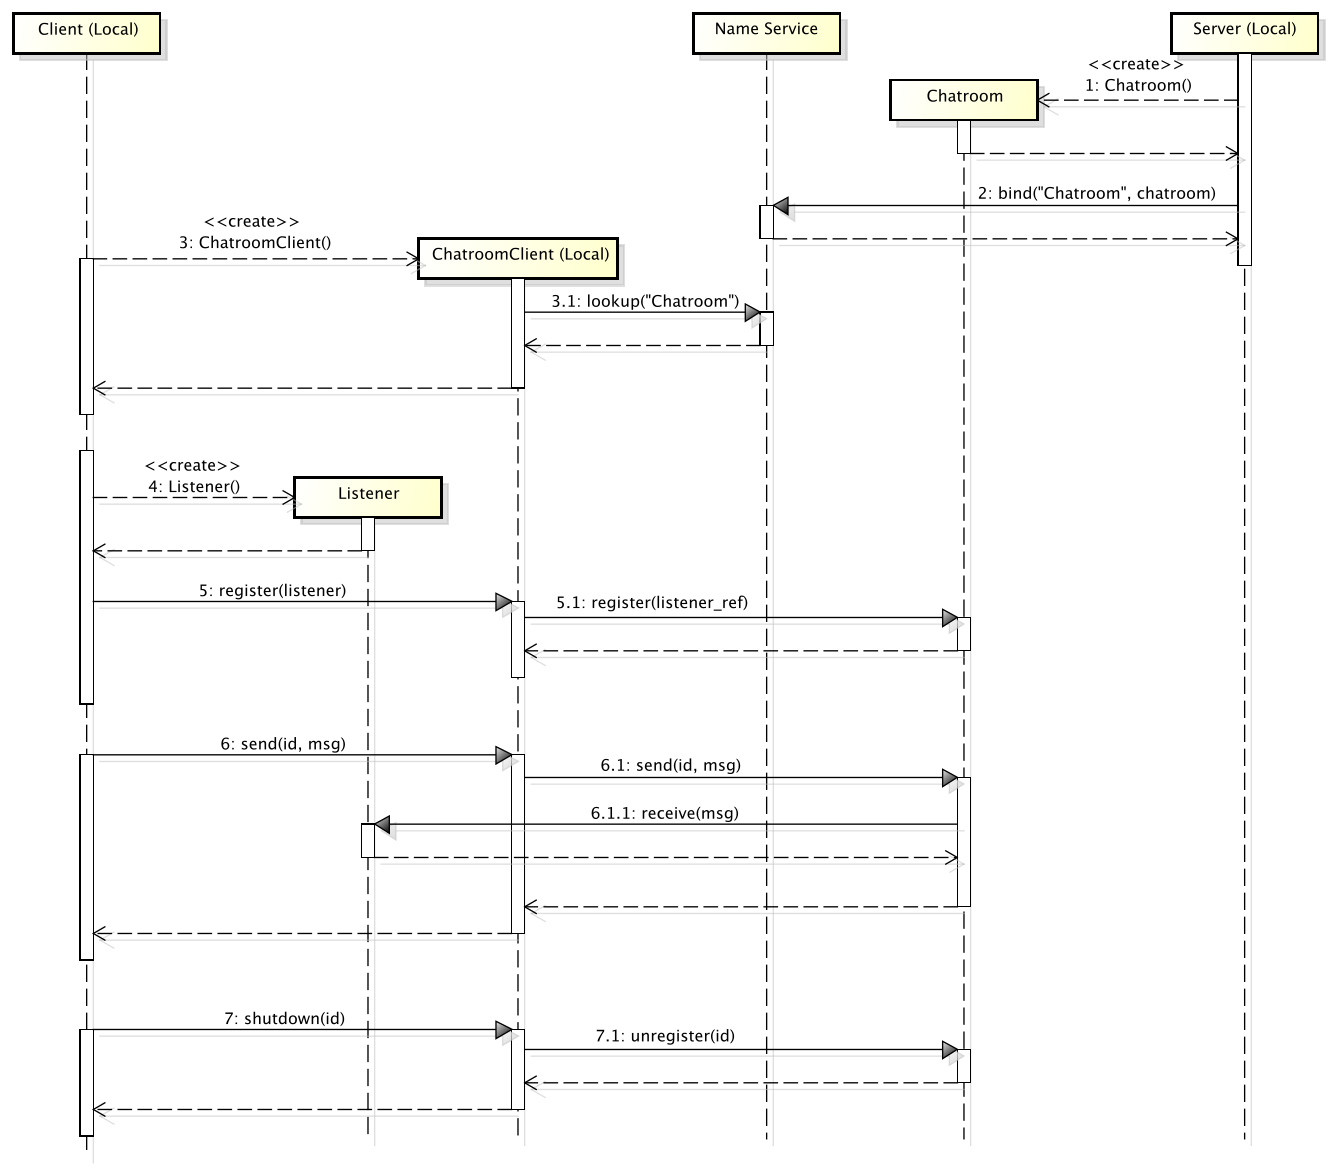
\includegraphics[width=0.8\linewidth]{images/sequence_diagram.pdf}
		\caption{Sequenzdiagramm des Kommunikationsablaufes der Anwendung}
		\label{broker}
	\end{center}
\end{figure}


\subsubsection{Server}
Die Implementierung der Server erfolgt in Java.
Im ersten Schritt werden daf\"ur die Interface Definitionen mithife eines Ant-Tasks generiert:

\begin{lstlisting}[language=XML, caption=Ant Task f\"ur die Generierung der IDL Interfaces]
<property name="src.dir" value="src" />
<property name="build.dir" value="build" />
<property name="classes.dir" value="${build.dir}/classes" />
<property name="doc.dir" value="doc" />
<property name="idl.dir" value="../idl" />
<property name="gen.dir" value="${build.dir}/generated" />
<property name="resources.dir" value="resources" />
<property name="jacorb.dir" value="/home/markus/opt/jacorb" />

<!-- Setzen des Classpaths von JacORB -->
<path id="jacorb.classpath">

	<!-- Setzen des Pfades zu, und inkludieren der Libaries -->
	<fileset dir="${jacorb.dir}/lib">
		<include name="*.jar" />
	</fileset>
</path>

<!-- Setzen des Classpaths des Projekts (classes Ordner in build) -->
<path id="project.classpath">
	<pathelement location="${classes.dir}" />
</path>

<!-- Definieren eines in einer bestimmten Klasse vorhandenen Tasks -->
<target name="idl.taskdef">
	<taskdef name="jacidl" classname="org.jacorb.idl.JacIDL"
		classpathref="jacorb.classpath" />
</target>

<!-- Generieren des aus dem idl File resultierenden Quellcodes  -->
<target name="idl" depends="idl.taskdef">
	<mkdir dir="${idl.dir}" />
	<jacidl srcdir="${idl.dir}" destdir="${gen.dir}" includes="*.idl"
		helpercompat="jacorb" includepath="${jacorb.dir}/idl/omg" />
</target>
\end{lstlisting}

In dem Ant-Script wird durch den entsprechenden Aufruf des JacORB IDL Compilers die Stubs und Skeletons des Interfaces generiert.

Danach muss am Server Chatroom implementiert werden, dies erfolgt durch Vererben der Klasse \texttt{ChatroomPOA}.
In dem Code finden sich keine speziellen, Corba spezifischen Elemente, es handelt es sich um eine simple Methoden, welche keine besondere Aufmerksamkert bed\"urfen.

Interessanter ist jedoch die tats\"achliche Implementierung des Servers und die Anbindung an Corba:
\begin{lstlisting}[language=Java, caption=Server Main Methode]
public static void main(String[] args)  {
    try {
        // Initialize the ORB
        ORB orb = ORB.init(args, null);
        System.out.println("Initialized ORB");

        //Instantiate Servant and create reference
        POA rootPOA = POAHelper.narrow(orb.resolve_initial_references("RootPOA"));
        ChatroomImpl chImpl = new ChatroomImpl();
        rootPOA.activate_object(chImpl);
        Chatroom chRef = ChatroomHelper.narrow(rootPOA.servant_to_reference(chImpl));

        //Bind reference with NameService
        NamingContext namingContext = NamingContextHelper.narrow(orb.resolve_initial_references("NameService"));
        System.out.println("Resolved NameService");
        NameComponent[] nc = { new NameComponent("Chatroom", "") };
        namingContext.rebind(nc, chRef);

        //Activate rootpoa
        rootPOA.the_POAManager().activate();

        //Start readthread and wait for incoming requests
        System.out.println("Server ready and running ....");

        orb.run();
    }	catch (Exception e)	{
        System.err.println("Es ist ein Fehler aufgetreten: " + e.getMessage());
        e.printStackTrace();
    }
}
\end{lstlisting}

In dem oberen Listing wird zun\"achst der ORB initalisiert und eine Referenz auf den Portable Object Adapter (POA) erzeugt, mithilfe dessen anschlie\ss end eine Instanz von \texttt{Chatroom} als Objektreferenz an den Namensdienst gebunden werden kann.
Dies geschieht in den Zeilen 7 bis 20.
Danach wird der ORB mit \texttt{orb.run()} gestartet.

Auch f\"ur die Ausf\"uhrung des Servers gibt es einen Ant-Task names \texttt{ant run-server}.

\subsubsection{Client}
Der Client, wird, wie zuvor bereits erw\"ahnt in Python implementiert, als Build Automation Tool kommt Make zum Einsatz.
In folgendem ist das akefile zusehen, die wichtigsten Targets sind hierbei das default Target \texttt{all}, welches die Python Bindings aus dem IDL generiert, sowie \texttt{run}, f\"ur das Starten des Clients.
\begin{lstlisting}[language=Make, caption=Makefile des Clients]
PYTHON         	= /usr/bin/python
PYTHON_PATH     = lib
CPPFLAGS      	= -g -c
OMNIIDL       	= /usr/local/bin/omniidl
IDL_DIR		    = ../idl
IDL_FILE	    = $(IDL_DIR)/chat.idl

all chat_idl.py: $(IDL_FILE)
	$(OMNIIDL) -bpython -Clib $(IDL_FILE)

run: chat_idl.py $(PYTHON)
# Start Naming service with command 'omniNames -start -always' as root
	PYTHONPATH=lib $(PYTHON) client.py markus -ORBInitRef NameService=corbaloc::127.0.0.1:2809/NameService

test: chat_idl.py $(PYTHON)
	PYTHONPATH=lib:. $(PYTHON) test/test_chatroomClient.py

clean clean-up:
	rm -rf *.o
	rm -rf *.hh
	rm -rf *SK.cc
	rm -rf server
\end{lstlisting}

Es wurde ein simples Kommandzeileninterface entwickelt, \"uber das der Benutzer nach der Registrierung des Clients am Server (bzw. nach der Anmeldung im Chatroom), Nachrichten senden kann.
Parallel dazu werden ankommende Nachrichten ausgegeben.
Wichtigster Teil ist die \texttt{ChatroomClient} Klasse, welche als Abstraktionsebene fungiert und die Kommunikation mit dem \texttt{Chatroom} Remoteobjekt \"ubernimmt
\begin{lstlisting}[language={Python}, caption=Chatroom Klasse des Clients als Abstraktionsebene zu CORBA]
class ChatroomClient:
    def __init__(self, orb_args):
        # Initialise the ORB
        self.orb = CORBA.ORB_init(orb_args)

        # Obtain a reference to the root naming context
        obj = self.orb.resolve_initial_references("NameService")
        rootContext = obj._narrow(CosNaming.NamingContext)

        self.poa = self.orb.resolve_initial_references("RootPOA")

        if rootContext is None:
            print "Failed to narrow the root naming context"
            sys.exit(1)

        # Resolve the name "test.my_context/ExampleEcho.Object"
        name = [CosNaming.NameComponent("Chatroom", "")]

        try:
            obj = rootContext.resolve(name)

        except CosNaming.NamingContext.NotFound, ex:
            print "Name not found"
            sys.exit(1)

        # Narrow the object
        self.chatroom = obj._narrow(chat.Chatroom)
        if self.chatroom is None:
            print "Object reference is not an chat.Chatroom"
            sys.exit(1)

        poa_manager = self.poa._get_the_POAManager()
        poa_manager.activate()

    def register(self, listener, listener_name):
        # get a remote object reference to the listener
        listener_ref = listener._this()
        # register the listener
        return self.chatroom.register(listener_ref, listener_name)

    def send(self, listener_id, msg):
        self.chatroom.send(listener_id, msg)

    def unregister(self, listener_id):
        self.chatroom.unregister(listener_id)
\end{lstlisting}
Im oberen Listing wurden die Methoden- und Klassenbeschreibungen entfernt um Platz zu sparen.
Im Konstruktor wird zun\"achst CORBA initialisiert und danach das \texttt{Chatroom} Objekt \"uber den Namensdienst abgerufen.
Desweiteren wird auch der POA (Protable Object Adapter) abgerufen, mit dem danach die Listener Objekte exportiert werden k\"onnen.
Die \"ubrigen Methoden \texttt{register(...)}, \texttt{unregister(...)} und \texttt{send(...)} sind nicht viel mehr als simple Wrapper \"uber das tats\"achliche \texttt{Chatroom} Objekt.
PyOmniORB ist multithreaded, der ORB Arbeitsthread wird bei Beendigung des Hauptthreads automatisch gestoppt.
Wichtig ist au\ss erdem, dass vor dem Beenden des Programmes noch der Listener entfernt wird, da der Server ansonsten Nachrichten an das nicht mehr existierende Objekt senden w\"urde.

Die Implementierung des Listeners ist sehr simpel, es muss lediglich von \texttt{chat\_\_POA.Listener} geerbt und die Methode \texttt{receive(...)} implementiert werden:

\begin{lstlisting}[language={Python}, caption=Simple Nachrichten Listener Implementierung ]
class ChatroomListener(chat\_\_POA.Listener):
    def receive(self, msg):
        print(msg)
\end{lstlisting}

\subsubsection{Ausf\"uhrung / Testcases}
F\"ur die Ausf\"uhrung sind 3 Komponenten erforderlich, diese werden wie folgt gestartet:
\begin{itemize}
    \item OMNI Naming Service: \texttt{sudo omniNames}
    \item Server: \texttt{ant run-server} (Im \texttt{server} Verzeichnis)
    \item Client: \texttt{make run} (Im \texttt{client\_python} Verzeichnis)
\end{itemize}

Dem Client wird als erster Parameter ein Name mitgegeben, der jeder Nachricht vorangestellt wird.
Dieser Name ist im Makefile hardcodiert um un\"otige Komplexit\"at zu vermeiden.

Auch wurden einige Testcases implementiert.
F\"ur die Ausf\"uhrung der Tests gibt es ebenfalls ein Make-Target im Client:

\texttt{make test}

Zuvor m\"ussen allerdings der Server und OmniNames gestartet werden.

\subsection{Arbeitszeit}
\renewcommand{\arraystretch}{1.5}
\begin{table}[H]
	\center
	\begin{tabular}{ | @{\hspace{3mm}} c @{\hspace{3mm}} | @{\hspace{3mm}} c @{\hspace{3mm}} | @{\hspace{3mm}} c @{\hspace{3mm}} | }
		\hline \textbf{T\"atigkeit} & \textbf{Datum} & \textbf{Dauer}\\ \hline\hline
		\textbf{Implementierung Aufgabe} & 13.5. & 4h\\ \hline
		\textbf{Implementierung + Protokoll} & 20.5. & 4h\\ \hline
        \textbf{Protokoll} & 26.5. & 4h\\ \hline
	\end{tabular}
	\caption{Arbeitszeitaufzeichnung}
	\label{methoden}
\end{table}
